\documentclass[10pt,twocolumn,letterpaper]{article}

\usepackage{cvpr}
\usepackage{times}
\usepackage{epsfig}
\usepackage{graphicx}
\usepackage{amsmath}
\usepackage{amssymb}
\usepackage{enumitem}
\usepackage{subcaption}

% Include other packages here, before hyperref.

% If you comment hyperref and then uncomment it, you should delete
% egpaper.aux before re-running latex.  (Or just hit 'q' on the first latex
% run, let it finish, and you should be clear).
\usepackage[breaklinks=true,bookmarks=false]{hyperref}

\cvprfinalcopy % *** Uncomment this line for the final submission

\def\cvprPaperID{****} % *** Enter the CVPR Paper ID here
\def\httilde{\mbox{\tt\raisebox{-.5ex}{\symbol{126}}}}

% Pages are numbered in submission mode, and unnumbered in camera-ready
%\ifcvprfinal\pagestyle{empty}\fi
\setcounter{page}{1}
\begin{document}

%%%%%%%%% TITLE
\title{Deep Dish : Deep Learning for Classifying Food Dishes}

\author{Abhishek Goswami\\
Microsoft\\
Redmond, WA\\
{\tt\small agoswami@microsoft.com}
% For a paper whose authors are all at the same institution,
% omit the following lines up until the closing ``}''.
% Additional authors and addresses can be added with ``\and'',
% just like the second author.
% To save space, use either the email address or home page, not both
\and
Haichen Liu\\
Dropbox\\
Seattle, WA\\
{\tt\small haichen@dropbox.com}
}

\maketitle
%\thispagestyle{empty}

%%%%%%%%% ABSTRACT
\begin{abstract}
   %The ABSTRACT is to be in fully-justified italicized text, at the top
   %of the left-hand column, below the author and affiliation
   %information. Use the word ``Abstract'' as the title, in 12-point
   %Times, boldface type, centered relative to the column, initially
   %capitalized. The abstract is to be in 10-point, single-spaced type.
   %Leave two blank lines after the Abstract, then begin the main text.
   %Look at previous CVPR abstracts to get a feel for style and length.
	
	We consider the problem of classifying food dishes. Food items have unique characteristics - they come in different colors and shapes, can be clustered into groups (e.g. fruits, vegetables), and can be combined in several ways to prepare a meal etc. This makes images of food dishes particularly interesting to classify. We show that convolutional neural networks are quite suitable for this task, and outperform traditional machine learning approaches in classifying food dishes.
		
\end{abstract}

%%%%%%%%% BODY TEXT
\section{Introduction}
\label{sec:introduction}

Over the past decade, the increasing use of wireless networking has fueled the 
use of wireless links to localize wireless clients in indoor spaces. This issue
is increasingly finding attention both from research and business communities 
because a perfect, general-purpose solution such as outdoor GPS has been elusive. Close scrutiny 
of available techniques reveal that more successful techniques require a substantial
`pre-deployment' effort by way of creating RF maps, for example. 
Technically, this is equivalent
to `training'. Fine grain RF map creation makes localization 
more accurate, but requires proportionately more effort.
On the other hand, any RF map is inherently device specific.
\emph{This pre-deployment burden that lacks generality
has made these localization techniques less appealing in practice.}  This paper develops a new machine-learning based localization algorithm, WiGEM,
that removes these limitations. 

%The received signal strength (RSS) based techniques are the most popular as commodity wireless devices are all capable of measuring RSS. 

Over time, two general localization approaches have emerged 
in literature -- (i) client-based approach~\cite{Haeberlen:2004:PRL:1023720.1023728, Gwon:2004:ECC:1023783.1023786, Youssef:2008:HLD:1399551.1399558, Chintalapudi:2010:ILW:1859995.1860016, Ladd:2002:RLS:570645.570674, Youssef:2003:WLD:826025.826335} and (ii)  infrastructure-based approach~\cite{Moraes:2006:CWL:1164783.1164799, Lim:2010:ZIL:1741400.1741464, Tao:2003:WLL:941311.941314, Krishnan04asystem}. In the client-based approach, the client device measures the RSS (received signal strength) as seen by it from various APs (access points). This information is used to localize the client. In the infrastructure-based approach, the network administrator can use simple sniffing devices (or APs doubling as sniffers) to monitor clients and record RSS from the client transmissions.  This sniffed RSS is used to localize the client. The infrastructure-based approach is more attractive for large scale deployment, because
any arbitrary client without any specific installed application can still localize itself
with the assistance of the infrastructure. It is also easier to deploy, manage and maintain. 

In the discussion that follows, we specifically focus on WiFi-based localization using
an infrastructure-based approach. WiFi is chosen because of the popularity of WiFi devices and WiFi-based WLAN systems. But the technique we develop is not specific to any link layer technology. At this point we also make a distinction between `learning' and `training'. By `learning' we actually mean unsupervised learning, whereby we automatically try to estimate our model parameters from unlabeled data. On the other hand, `training' is akin
to supervised learning that in our scenario leads to substantial limitations as discussed next.


%
%alluring for large-scale deployments, especially if building and maintaining the model can be automated. Moreover, such techniques perform location estimation without requiring hardware and/or software changes on the client device, which make them particularly attractive.
%
%
%
%Recent research has recognized this issue; however the proposed technique is not universally applicable~\cite{}. The goal of our work 
%to develop a unsupervised learning technique that works without any training
%
%the need for location-aware pervasive computing applications in indoor environments. Traditional GPS-based techniques have problems working indoor which make them unattractive for such fine-grained indoor localization. On the other hand, indoor wireless LAN (WLAN) technologies, which have been enthusiastically and widely adopted in enterprises and homes, give us interesting features like Received Signal Strength(RSS), Angle of Arrival(AoA) etc for robust location estimation. Received signal strength (RSS) is particularly interesting because current commercial hardware can be used to extract the signal strength of wireless frames being transmitted by a Wi-Fi device. 
%
%Several techniques [x, y, x] have demonstrated the viability of using the RSS metric for location estimation.   It is interesting to note here that most of these location-estimation systems can essentially be categorized in two distinct ways : a client-based approach [p, q, r] and an infrastructure-based approach [a, b, c]. In the client-based approach, the client device measures the signal strength as seen by it from various AP(Access Point). This information is used to locate the client. In the infrastructure-based approach, the network administrator can use simple sniffing devices (or APs masquerading as sniffers) to monitor clients and extract the RSS from the tx-client.  This sniffed information is used to locate the client. Considering ease of management, provisioning, security, deployment,  maintenance etc, the infrastructure-based model seems alluring for large-scale deployments, especially if building and maintaining the model can be automated. Moreover, such techniques perform location estimation without requiring hardware and/or software changes on the client device, which make them particularly attractive.
%

\subsection{Limitations of Training}
\label{subsec:limitationsoftraining}

In the existing indoor WiFi localization solutions, the first phase is a pre-deployment `offline phase' or training phase aimed at building detailed RF maps or RF propagation models based on a survey of the target area. The second phase is the `online phase', where a localization algorithm is used to provide a location estimate for an observed set of RSS measurements from the mobile device being localized. There are three major drawbacks of this general approach. 
\begin{enumerate}
\item
The device used during the `offline phase' may differ from the target device in the `online phase'. Unmodeled hardware devices operating at different transmit power levels can introduce significant variations in the signal patterns between the training device and the target device. This adversely affects the accuracy of location estimation \cite{Tsui:2009:ULS:1741410.1741596}. Experiments described later in this paper indicate how hardware variations between four common commodity WiFi devices can significantly degrade the accuracy of two commonly used localization algorithms. 
\item
The `offline phase' itself involves labor-intensive sampling of signal strength values at discrete locations in the target space. Again, experiments show that location accuracy depends significantly on the granularity of the training locations. If the training locations are sparse, the location estimates become substantially poorer.
\item
Static models built during the `offline phase' cannot counter time varying phenomena like movement of people, changing occupancy and surroundings etc. Most 
`killer' applications of indoor localization would be in large shopping malls, airports, 
convention centers etc., where such changes would be routine. 
On the other hand, due to the reason 2 above, such models are difficult to update regularly. 
\end{enumerate}

\subsection{Approach}

We propose WiGEM, a novel {\bf Wi}reless
localization algorithm that uses the {\bf G}aussian Mixture Model (GMM) and employs {\bf E}xpectation 
{\bf M}aximization (EM) to estimate the model parameters. 
The model is initialized 
using  a standard radio propagation model~\cite{Rappaport:2001:WCP:559977, Molkdar91} 
and typical constraints that exist between the received signal strengths for different transmit 
power levels at the same 
location.

WiGEM leverages the infrastructure based approach 
while eliminating any `pre-deployment' effort. Packet transmissions made by a client are received on stationary sniffers 
(or APs doubling as sniffers) that extract the RSS and MAC id of the target client and report this information to a 
central localization server. Using this information, WiGEM builds a model for the target device and provides 
a location estimate. The estimate can be made available to the client via a simple web-based
application,  for example, depending on the intended application. But this is not a part
of the current work. 



WiGEM provides several key benefits by eliminating the `offline phase'. First, building a model for each target device effectively addresses the hardware variance problem. Thus, WiGEM can be used across heterogeneous devices, each operating at different power levels.  Second, zero `pre-deployment' effort makes WiGEM particularly attractive for large indoor spaces. Third, WiGEM is a purely online algorithm: the model parameters get updated and modified based on real-time RSS observations. As such, WiGEM is able to adapt to dynamic changes in the target space.

The remainder of the paper is organized as follows. In Section~\ref{sec:relatedwork}, we survey related work in Indoor Localization. In Section~\ref{sec:problemformulation} we introduce WiGMM, the modeling approach we use to localize a target device, and discuss the parameters of the model. In Section~\ref{sec:emalgorithm} we discuss the EM algorithm, which is used to estimate the parameters of our model. Section~\ref{sec:experimentmethodology} provides details on the experiment methodology and Section~\ref{sec:evaluation} presents the experimental results obtained from two different testbeds. In Section~\ref{sec:discussion} we discuss WiGEM and identify items for future work. Finally, we present our conclusions in Section~\ref{sec:conclusions}.

% \textbf{Our results of deploying GEM in two different office buildings are promising. We specifically note that when measurements made using one device are used to localize a different device,  GEM is seen to perform better that RF signal map based techniques like RADAR[x] and Probabilistic[y]
% }
\section{Related Work}
\label{sec:relatedwork}

In this section we provide a brief overview of some
of the fundamental techniques in the field of indoor wireless 
localization. In passing, we also point out their limitations
with respect to the proposed WiGEM technique. \\

%Over the past two decades, this field has seen tremendous push, both from the research community and from industrial circles. The advent of pervasive and mobile computing has fueled tremendous interest in this field in recent years.  \\

\noindent {\bf Calibration-free techniques:} An indoor path-loss propagation model essentially forms the bedrock for these techniques. In RADAR, Bahl {\it et al} \cite{Bahl00radar:an} 
provide a indoor radio propagation model to calculate RSS at various locations in the building based on distance, number of walls etc. The nearest neighbor in signal space (NNSS) metric is then used to estimate the location of the  mobile user by matching the observed RSS to the theoretically computed signal strength values at these locations. In \cite{Moraes:2006:CWL:1164783.1164799, Lim:2010:ZIL:1741400.1741464} the authors describe sniffer based techniques for localization based on propagation models. Moraes {\it et al} \cite{Moraes:2006:CWL:1164783.1164799} use a naive propagation model to generate a `radio propagation map' (RPM) at each sniffer. They use RSS measurements between the sniffers and a `reference AP' (APRef) to reconstruct the RPM, either periodically or when there are significant variations in the RSS. A probabilistic model is then used to compute a location estimate.  Lim {\it et al}~\cite{Lim:2010:ZIL:1741400.1741464} consider online measurements of RSS between 802.11 APs and between a client and its neighboring APs, to create a mapping between the RSS measure and the actual geographic distance. TIX~\cite{Gwon:2004:ECC:1023783.1023786} uses a similar setting whereby inter-AP and client-AP RSS measurements are used to perform linear interpolation for estimating the RSS at distinct locations in the target space. Madigan {\it et al}~\cite{Madigan05bayesianindoor} propose a client-based scheme that uses a Bayesian hierarchical graphical model. By making the assumption that different access points behave similarly, they develop a model which avoids the need to know the location of the training points. {\it While most of these schemes are designed to be responsive to real time changes in the environmental dynamics of the target space, none of them model variations in client hardware and transmission power, factors which can significantly degrade the accuracy estimates of RSS based WiFi localization schemes.} \\

\noindent {\bf Techniques that build RF signal maps:} Several client-based schemes and infrastructure-based schemes rely on RF signal maps for localization.  The basic approach is to have a pre-deployment `offline phase' or training phase aimed at building detailed RF maps or RF propagation models based on a survey of the target area. The client device is then localized by matching the observed RSS against the signal map. RADAR-empirical \cite{Bahl00radar:an} was one of the first RF-based schemes to use this model. In recent years, a number of probabilistic techniques \cite{Youssef:2008:HLD:1399551.1399558, Ladd:2002:RLS:570645.570674, Haeberlen:2004:PRL:1023720.1023728} have been proposed to enhance the robustness of localization. For the probabilistic techniques, the `offline phase' corresponds to the construction of conditional  probability distributions that map signal intensities to locations on a map.  %Thus, we first build up a {\it signal map} database for the area being covered. 
During the location determination phase, given a real-time RSS signature,  a probabilistic inference algorithm is used to select the most likely location from all possible locations in the target space. As mentioned in Section~\ref{subsec:limitationsoftraining}, \emph{these techniques require considerable `pre-deployment' training effort, are difficult to maintain and update with changing dynamics in the target space and are inherently susceptible to the hardware variance problem~\cite{Tsui:2009:ULS:1741410.1741596}. }\\


\noindent{\bf Prior work on hardware variance:} Tsui {\it et al}~\cite{Tsui:2009:ULS:1741410.1741596} observe that hardware variance can significantly degrade the positional accuracy of RSS-based Wi-Fi localization systems. In fact, they note that the hardware variance problem is not limited to differences in the WiFi chipsets used by training and tracking devices, but also occurs when the same Wi-Fi chipsets are connected to different antenna types and/or packaged in different encapsulation materials. The authors introduce an intermediate `online adjustment' phase where they use unsupervised learning to construct a signal transformation function between the training device and a new target device. Prior work on hardware variance \cite{Haeberlen:2004:PRL:1023720.1023728} observe a linear relationship between the RSS mappings of several commodity Wi-Fi cards and suggest a manual calibration effort to identify this relationship between different cards. {\it The ever-increasing number of WiFi chipsets, antennas and encapsulating materials make this manual adjustment effort impractical in real-world deployments}. 

Tao {\it et al}~\cite{Tao:2003:WLL:941311.941314} have an interesting take on unmodeled hardware and transmission power variations.  They observe that RSS is linearly proportional to transmission power. Based on the difference in signal strength between every pair of sniffers, they suggest a weighted heuristic to give a location estimate for a target RSS fingerprint.\\

\noindent{\bf WiGEM compared to prior work:} The major contribution of this work is to develop an algorithm, WiGEM, that eliminates the expensive `training' phase. 
While a similar attempt has also been made in a recent work~\cite{Chintalapudi:2010:ILW:1859995.1860016}, this technique depends on the availability of GPS feed in some indoor
locations, more the better. WiGEM does not depend on availability of GPS. 
%
WiGEM can adapt to variations in transmit power across heterogeneous devices, which makes it particularly suitable for infrastructure-based localization schemes. The algorithm also `learns on the go' and thus can factor in real-time changes in the environmental dynamics of the target space. 

\section{Methods}
\label{sec:methods}

Image classification is the task of assigning a single label to an image (or rather an array of pixels that represents an image) from a fixed set of categories. A complete pipeline for this task is as follows:
\begin{itemize}[noitemsep]
\item \textbf{Input} : A set of $N$ images, each labeled with one of $K$ different classes. This data is referred to as the \textit{training set}.
\item \textbf{Learning} (aka Training) : Use the \textit{training set} to learn the characteristics of each class. The output of this step is a \textit{model} which will be used for making predicions.
\item \textbf{Evaluation}  : Evaluate the quality of the \textit{model} by asking it to make predictions on a new set of images that it has not seen before (also referred to as the \textit{test set}). This evaluation is done by comparing the true labels (aka ground truth) of the \textit{test set} with the predicted labels output by the learned \textit{model}.
\end{itemize}

The formal approach for solving the problem of image classification can be broken down into several key components which we discuss next.

\subsection{Score Function}
\label{subsec:scorefunction}

The score function maps the raw data to class scores. For a linear classifier, the score function can be defined as: 
\begin{align}
f(\boldsymbol{x_{i}}, \boldsymbol{W}, \boldsymbol{b}) = \boldsymbol{W} \boldsymbol{x_{i}} + \boldsymbol{b}.\label{eqn:scorefunction}
\end{align}

where $\boldsymbol{x_{i}}$ represents the input image. The matrix $\boldsymbol{W}$, and the vector $\boldsymbol{b}$ are the parameters of the function, and represent the weights and bias respectively.

In image classification, the score function takes an image ${\boldsymbol {x_{i}}}$ and computes the vector $f(\boldsymbol{x_{i}}, \boldsymbol{W})$ of the raw class scores (which we abbreviate as ${\boldsymbol {s}}$). So, given an image ${\boldsymbol {x_{i}}}$, the predicted score for the j-th class is the j-th element in $\boldsymbol{s}$ : $\boldsymbol{s}_{j} = f(\boldsymbol{x_{i}}, \boldsymbol{W})_{j}$. We use the  class scores from our training data to compute the loss.

\subsection{Loss Function}
\label{subsec:lossfunction}

The loss function quantifies the match between the predicted \textit{scores} and the ground truth labels in the training data. The loss function (also referred to as the cost function or objective) can be viewed as the unhappiness of the predicted scores output by the score function. Intuitively, the loss would be low if the predicted scores match the training data labels closely. Otherwise the loss would be high. Next, we discuss the two common classifiers with details about their respective loss functions. 

\subsection{Classifiers}
\label{subsec:classifiers}

In this section we discuss two common classifiers that are often used in image classification tasks: the \textbf{SVM Classifier} and the \textbf{Softmax Classifier}. For both of them the function mapping the input image $\boldsymbol{x_{i}}$ to the raw class scores $\boldsymbol{s} = f(\boldsymbol{x_{i}}, \boldsymbol{W})$ remains the same. But the Softmax classifier has one additional step : it uses the softmax function to squash the raw scores in $\boldsymbol{s}$ into a vector of values between zero and one, that sum to one.  We discuss the details of each classifier below.

\subsubsection{SVM Classifier}
\label{subsubsec:svmclassifier}

The SVM classifier uses the \textit{hinge loss} (also referred to as \textit{max-margin loss}, or \textit{SVM loss}). For the i-th example in our data, the \textit{hinge loss} is given as:

\begin{align}
L_{i} = \sum_{j \neq y_{i}} \max(0, \boldsymbol{s}_{j} - \boldsymbol{s}_{y_{i}} + \Delta).\label{eqn:svmloss}
\end{align}

where $\Delta$ is a hyperparameter which represents that the SVM loss function in equation~\ref{eqn:svmloss} wants the score of the correct class $\boldsymbol{y_{i}}$ to be larger than the incorrect class scores by at least $\Delta$. Otherwise we incur loss. 

\subsubsection{Softmax Classifier}
\label{subsubsec:softmaxclassifier}

The Softmax classifier uses the \textit{cross entropy loss} (also referred to as \textit{softmax loss}). For the i-th example in our data, the \textit{cross entropy loss} is given as:

\begin{align}
L_{i} =  - \log \frac {e^{f_{y_i}}} {\sum_{j} e^{f_{j}}}.\label{eqn:softmaxloss}
\end{align}

where $f_{j}$ means the j-th element of the vector of class scores $f$. Note that the softmax classifier uses the softmax function to squash the raw class scores ${\boldsymbol {s}}$ into normalized positive values that sum to one, so that the cross entropy loss can be applied. The \textbf{softmax function} can be represented as:

\begin{align}
f_{j} (z) =  \frac {e^{z_j}} {\sum_{k} e^{z_{k}}}.\label{eqn:softmaxfunction}
\end{align}

It takes a vector of real-valued scores (in z) and squashes it to a vector of values between zero and one, that sum to one.

\subsection{Total Loss}
\label{subsec:totalloss}

For both the SVM Classifier and the Softmax Classifier, the full loss for the dataset is the mean of $L_{i}$ over all training examples, together with a regularization term, $R(W)$

\begin{align}
L =  \frac {\sum_{i} L_{i}} {N} +  \lambda R(W).\label{eqn:totalloss}
\end{align}

where $N$ represents the total number of images in the training set. $\lambda$ is a hyperparameter, often referred to as \textit{regularization strength}. The loss function lets us quantify the quality of any particular set of parameters in our model, the lower the loss the better. We next discuss strategies of how to minimize the loss.

\subsection{Optimization}
\label{subsec:optimization}

Optimization is the process of finding the set of parameters of our model that minimize the total loss, defined in equation~\ref{eqn:totalloss}

The core principle behind optimization techniques is to compute the \textbf{gradient} of the loss with respect to the parameters of the model. The gradient of a function gives the direction of steepest ascent. One way of computing the gradient efficiently is to compute the gradient analytically using a recursive application of the \textbf{chain rule}. This technique is called \textbf{backpropagation}~\cite{lecun2012efficient} and it allows us to efficiently optimize arbitrary loss functions. These loss functions  may be expressing different kinds of network architectures (e.g. fully connected neural networks, convolutional networks etc). Backpropagation is our tool of choice for computing the gradients in all such cases.  

\subsubsection{Parameter Updates}
\label{subsubsec:parameterupdates}
   
Once the analytic gradient is computed using backpropagation, the gradients are used to perform a parameter update. There are several approaches for performing the update that have been proposed in literature: SGD~\cite{bottou2010large}, SGD+Momentum~\cite{qian1999momentum, sutskever2013importance}, Nesterov Momentum~\cite{nesterov1983method}, Adagrad~\cite{duchi2011adaptive}, RMSprop~\cite{hinton2012neural}, Adam~\cite{kingma2014adam} etc.

%-------------------------------------------------------------------------
\section{Dataset and Features}
\label{sec:datasetandfeatures}

We start with a discussion about our data collection methodology. We then present details about the data pre-processing steps. Finally we round up this section with details about our dataset.

We provide some details about our dataset below.

\subsection{Data Collection}
\label{subsec:datacollection}

We collected our dataset using the Google Image Search~\cite{googleimagesearch} and the Bing Image Search API~\cite{bingimagesearchapi}. We also explored the use of ImageNet~\cite{imagenet} and Flickr~\cite{flickr} for collecting images. However, we found the images from Google and Bing to be much more representative of the classes they belonged to, compared to the images from ImageNet and Flickr. ImageNet and Flickr seem to have a lot of spurious images (images which clearly do not belong to the class). Hence we decided to use the images we could collect from Google and Bing.

\subsection{Pre-Processing Steps}
\label{subsec:preprocessingsteps}

We re-sized all of our images to have height, width and channel dimensions of 32, 32 and 3 respectively. This was done primarily for computational efficiency in performing our experiments. We filtered out images which we were unable to resize to our specified height, width and channel requirements. Unfortunately, this meant losing approx ~10\% of the data from our original dataset. Figure~\ref{fig:imgsburgerpizza} shows a two sample images from our dataset. As a part of pre-processing, we also subtract the mean image from all the images in our dataset. The mean image is computed using the image mean of the training data

\subsection{Dataset Details}

\begin{table}
\begin{center}
\begin{tabular}{|l|c|}
\hline
Dataset & Num of Images \\
\hline
Train & 18,927 \\
Validate & 5,375 \\
Test & 2,682 \\
\hline
\end{tabular}
\end{center}
\caption{Dataset split for train, validation and test sets.}
\label{table:datasplitdetails}
\end{table}

After the pre-processing steps described in Section~\ref{subsec:preprocessingsteps} we had a total of 26,984 images. We then split our dataset randomly into 3 disjoint sets: Train(70\% approx.), Validate(20\% approx.) and Test(10\% approx.). Table~\ref{table:datasplitdetails} provides a count of the number of images in each set.

Currently our dataset has 20 classes.  This corresponds to 20 popular food dishes from around the world. Table~\ref{table:classdistribution} shows the class label distribution of the dataset. The distribution of the number of images in each class is mostly uniform. 

\begin{table}
\begin{center}
\begin{tabular}{|l|c|}
\hline
Food Item & Number of Images \\
\hline\hline
dumplings & 1,091\\
dal & 1,031\\
ramen & 1,023\\
icecream & 1,021\\
naan & 1,020\\
sushi & 1,020\\
cordonbleu & 1,018\\
pasta & 1,002\\
lasagna & 971\\
friedrice & 966\\
roastturkey & 930\\
padthai & 919\\
burger & 912\\
samosa & 897\\
burrito & 888\\
pizza & 885\\
bratwurst & 876\\
biryani & 865\\
sandwich & 847\\
fries & 745\\
\hline
\end{tabular}
\end{center}
\caption{Class distribution}
\label{table:classdistribution}
\end{table}


%-------------------------------------------------------------------------
\section{Evaluation Results}
\label{sec:evaluationresults}

In this section we discuss our experiments and results. We chose accuracy as our evaluation metric when comparing different models. For brevity, we are reporting the accuracy numbers to two decimal places. 

For Section~\ref{subsec:linearclassifiersonrawimagepixels}, Section~\ref{subsec:neuralnetworksonrawimagepixels} and Section~\ref{subsec:imagefeatures} we re-purposed code from assignments 1 and 2 in Stanford University's Spring 2017 course, CS231N: Convolutional Neural Networks for Visual Recognition~\cite{cs231n}. For Section~\ref{subsec:convolutionalnetworks} and Section~\ref{subsec:transferlearning}, we use TensorFlow~\cite{abadi2016tensorflow} for training our convolutional network models.

\begin{table*}[h!]
\begin{center}
\begin{tabular}{|l|c|c|}
\hline
Modeling Approach & Best Validation Accuracy & Test Set Accuracy \\
\hline\hline
Linear SVM on raw image pixels & 0.18 & 0.16 \\
Five layer fully connected neural net on raw image pixels & 0.19 & 0.18 \\
Linear SVM on image features & 0.21 & 0.22 \\
Two layer neural net on image features & 0.26 & 0.27 \\
Training a Convolutional Network from scratch  & 0.40 & 0.40 \\
Transfer Learning (by fine tuning a VGG model) & 0.46 & 0.45 \\
\hline
\end{tabular}
\end{center}
\caption{Summary of results across different modeling approaches.}
\label{table:accuracyresults}
\end{table*}

\subsection{Linear classifiers on raw image pixels}
\label{subsec:linearclassifiersonrawimagepixels}

%\begin{figure} 
%\centering
%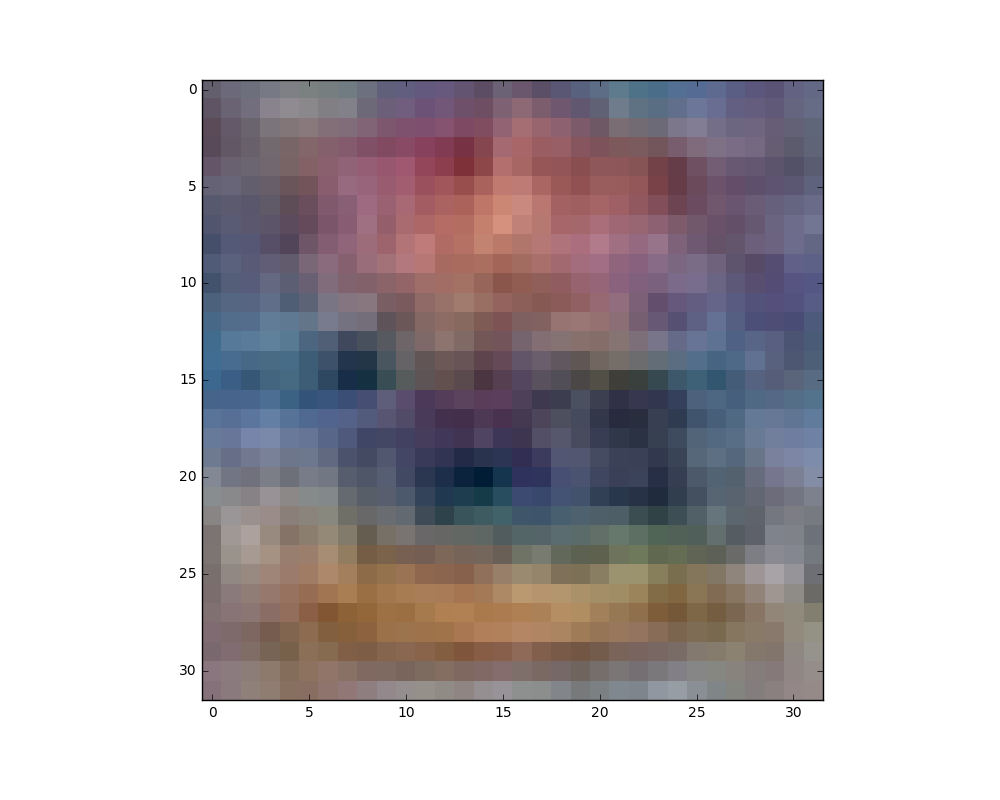
\epsfig{file=Figs4Paper/_final/svm_learnedweights_burger.eps, height=1.25in, width=1.6in} 
%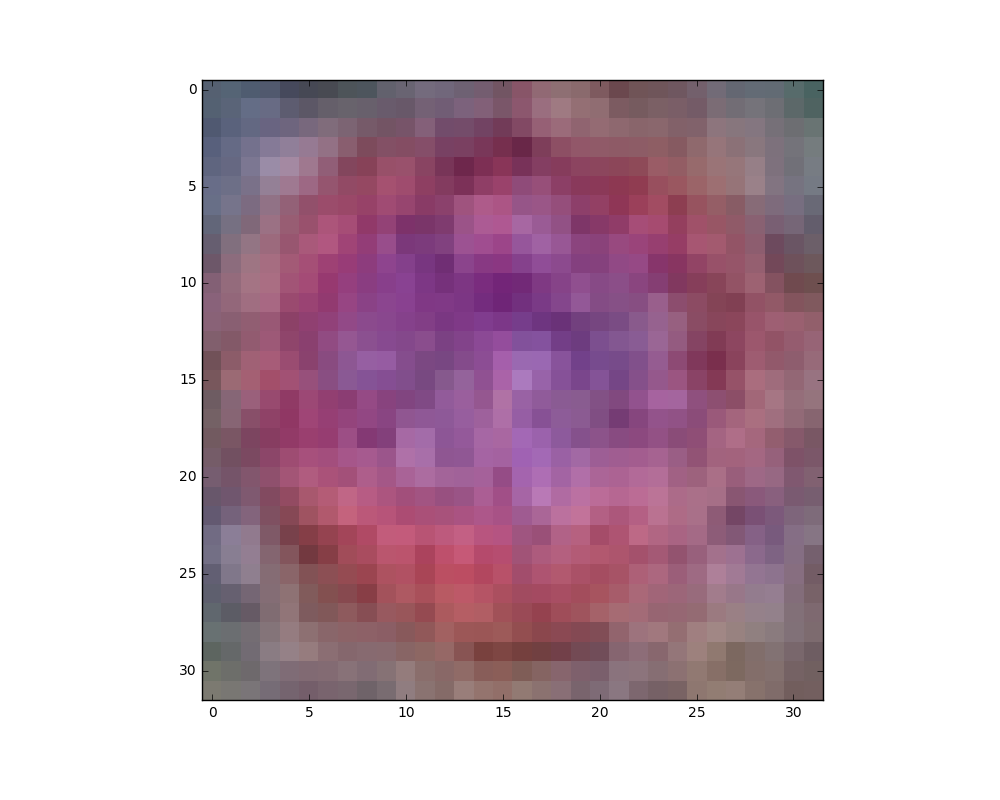
\epsfig{file=Figs4Paper/_final/svm_learnedweights_pizza.eps, height=1.25in, width=1.6in}
%\caption{Visualizing the weights learned by the SVM model for the burger and pizza classes}
%\label{fig:learnedweightsburgerpizza}
%\end{figure}

\begin{figure}[ht!]
    \centering
    \begin{subfigure}{.4\linewidth}
        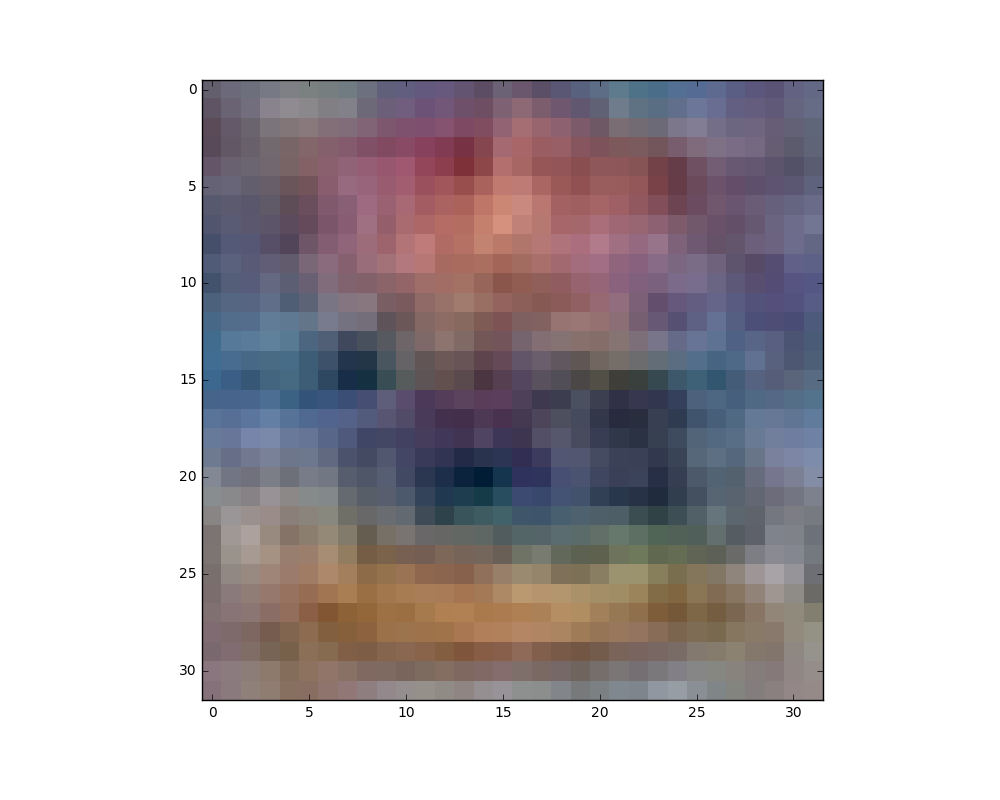
\includegraphics[height=1.25in, width=1.6in]{Figs4Paper/_final/svm_learnedweights_burger.eps}
        \caption{burger}
    \end{subfigure}
    \hskip2em
    \begin{subfigure}{.4\linewidth}
        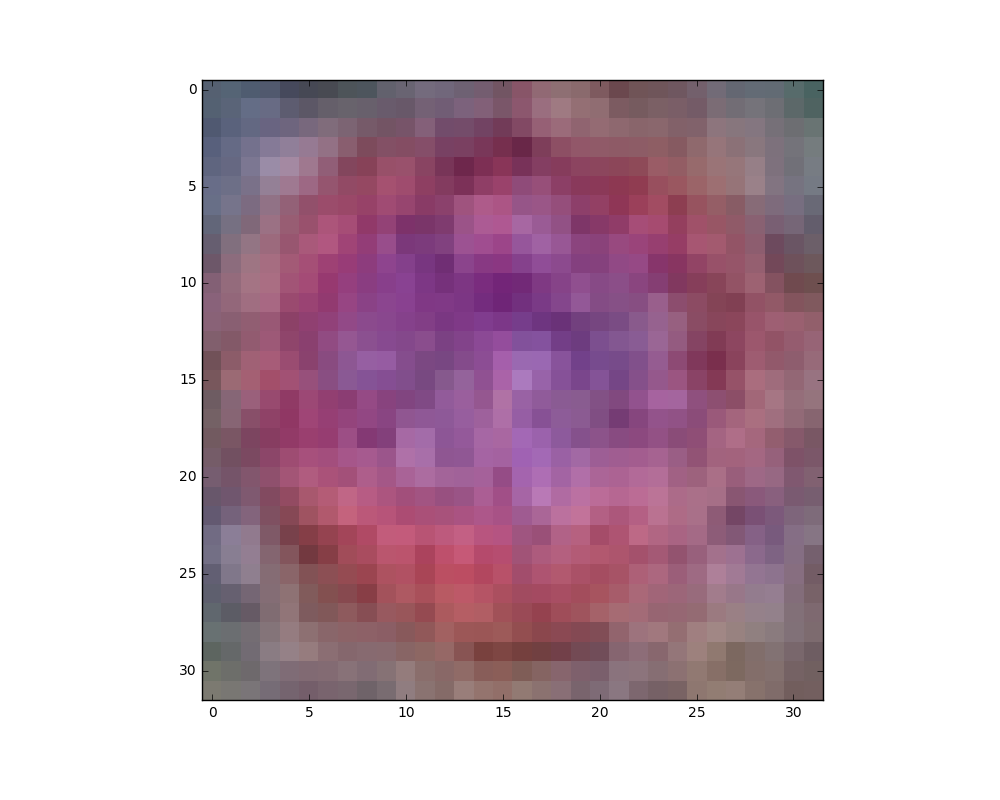
\includegraphics[height=1.25in, width=1.6in]{Figs4Paper/_final/svm_learnedweights_pizza.eps}
        \caption{pizza}
    \end{subfigure}
    \caption{Visualizing the weights learned by the SVM model}
		\label{fig:learnedweightsburgerpizza}
\end{figure}


To set our baseline, we first use a linear classifier using raw image pixels as features. For this we tried out both a SVM classifier and a Softmax classifier. The best validation accuracy of 0.18 was achieved using the SVM classifier with a learning rate 1e-07 and regularization strength 2.5e+04. The corresponding test set accuracy was 0.16.

One interpretation of a linear classifier is that of a \textit{template match}, where each row of the learned weights matrix corresponds to a template for the corresponding class. Figure~\ref{fig:learnedweightsburgerpizza} shows the learned weights for the burger and pizza classes in our dataset. We note that both the templates match our intuition; the burger contains a lot of brown pixels, the pizza has a round shape and contains a lot of red pixels at the center.   

\subsection{Neural networks on raw image pixels}
\label{subsec:neuralnetworksonrawimagepixels}

\begin{figure}[h!]
\centering
  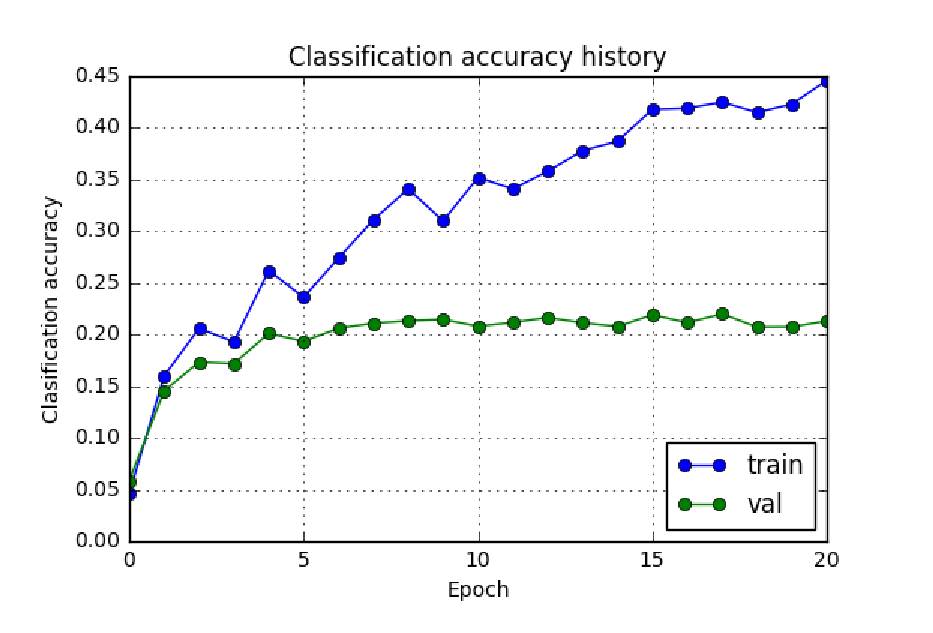
\epsfig{file=Figs4Paper/_final/fcfivelayer_rawpixels_classificationaccuracy.eps, height=1.5in, width=2.5in}
  \caption{Classification accuracy history of a fully connected five layer neural network using raw image pixels}
  \label{fig:fcfivelayerrawpixelsclassificationaccuracy}
\end{figure}

The next set of models we tried out were fully connected neural networks, again using raw image pixels as features.  Our network architecture was a six layer fully-connected network. Each of the five hidden layers had 100 neurons each. We used ReLU nonlinearity, and a softmax loss function. Below we note some interesting observations from training these models.

\begin{itemize}[noitemsep]
\item Batch normalization was~\cite{ioffe2015batch} \textbf{very useful} in training our model. Without batch normalization our model was performing quite poorly.
\item The best validation accuracy of 0.19 was achieved using the \textbf{Adam}~\cite{kingma2014adam} update rule with a learning rate of 1e-03. The test set accuracy was 0.18   
\end{itemize}

Figure~\ref{fig:fcfivelayerrawpixelsclassificationaccuracy} shows the classification loss history for the training and validation sets over 20 epochs while training this network.

\begin{figure*}[h!]
\centering
	\fbox{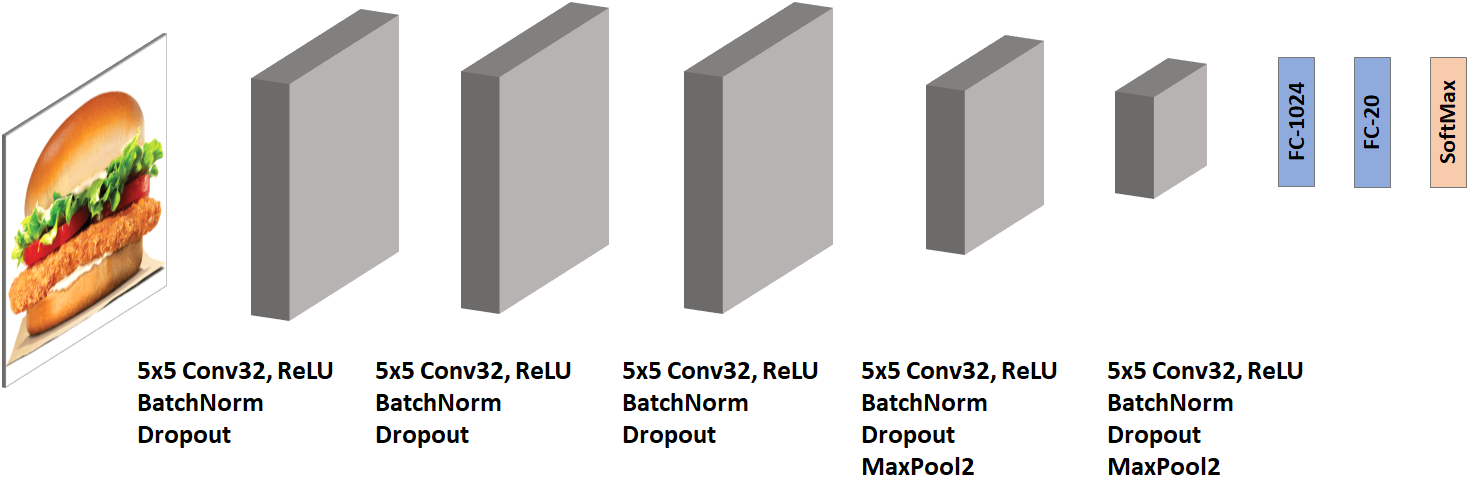
\includegraphics[width=12cm]{Figs4Paper/_final/convnet_architecture.eps}}
  \caption{Convolutional network architecture}
  \label{fig:convnetarchitecture}
\end{figure*}

\subsection{Image features}
\label{subsec:imagefeatures}


\begin{figure}[h!]
\centering
  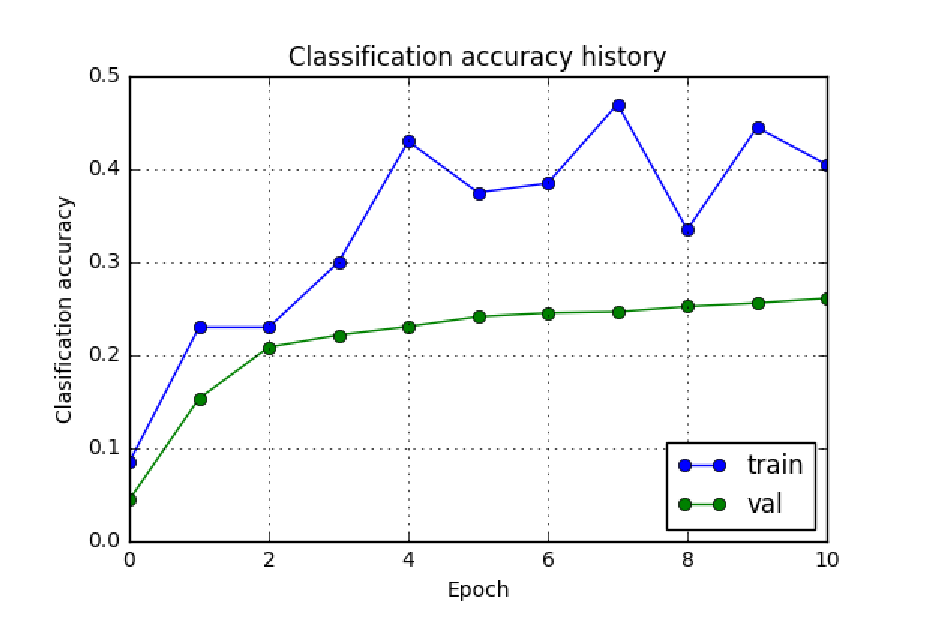
\epsfig{file=Figs4Paper/_final/imagefeatures_fctwolayer_classificationaccuracy.eps, height=1.5in, width=2.5in}
  \caption{Classification accuracy history of a fully connected two layer neural network using image features}
  \label{fig:imagefeaturesfctwolayerclassificationaccuracy}
\end{figure}

We did a set of experiments using features extracted from the images. For featurizing each image, we compute a Histogram of Oriented Gradients (HOG) as well as a color histogram using the hue channel in HSV color space. We form our final feature vector for each image by concatenating the HOG and color histogram feature vectors. This gives us a total of 155 features for each image. Below we summarize the results using image features with a SVM and a Two Layer Fully Connected Neural Network classifier.

\begin{itemize}[noitemsep]
\item Using the images features with a linear SVM classifier we were able to get a validation accuracy of 0.21, using SGD with a learning rate of 1e-03 and regularization strength of 1e+00
\item Using the images features with a Two Layer Fully Connected Neural Network gave much better performance. We got the best validation accuracy of 0.26 while using SGD as our update rule with a learning rate of 0.9, learning rate decay of 0.8 and regularization strength 0. The corresponding test set accuracy was 0.27   
\end{itemize}

Figure~\ref{fig:imagefeaturesfctwolayerclassificationaccuracy} shows the classification loss history for the training and validation sets over 10 epochs while training the Two Layer Fully Connected Neural Network classifier with image features.

\subsection{Convolutional Networks}
\label{subsec:convolutionalnetworks}

Using Convolutional Networks we were able to get the validation and test set accuracy of 0.40 each. Figure~\ref{fig:convnetarchitecture} shows the architecture we used. Below we note some of the things we tried out.

\begin{itemize}[noitemsep]
\item Batch normalization~\cite{ioffe2015batch} was quite useful in training our model.
\item For the weights in our network, using Xavier initialization~\cite{glorot2010understanding} helped.
\item Dropout~\cite{hinton2012improving, srivastava2014dropout} (with keep probability 0.75) helped improve the validation accuracy from 0.38 to 0.40. 
\item We kept the number of filters fixed at 32. 
\item We tried different sized filters (3x3, 5x5 and 7x7) but they did not help much. So we fixed the filter size at 5x5.
\item For the first three conv layers we preserve the height and width dimensions. For the fourth and fifth conv layers, we used max pooling with stride 2 (across both height and width).
\item After the five conv layers, we added two fully connected layers with 1024 and 20 neurons respectively. 
\item For the last layer we use softmax with cross entropy loss. 
\item The best validation accuracy of 0.40 was achieved using the \textbf{Adam}~\cite{kingma2014adam} update rule with a learning rate of 1e-04. The test set accuracy was 0.40. 
\end{itemize}

\begin{figure}[h!]
\centering
  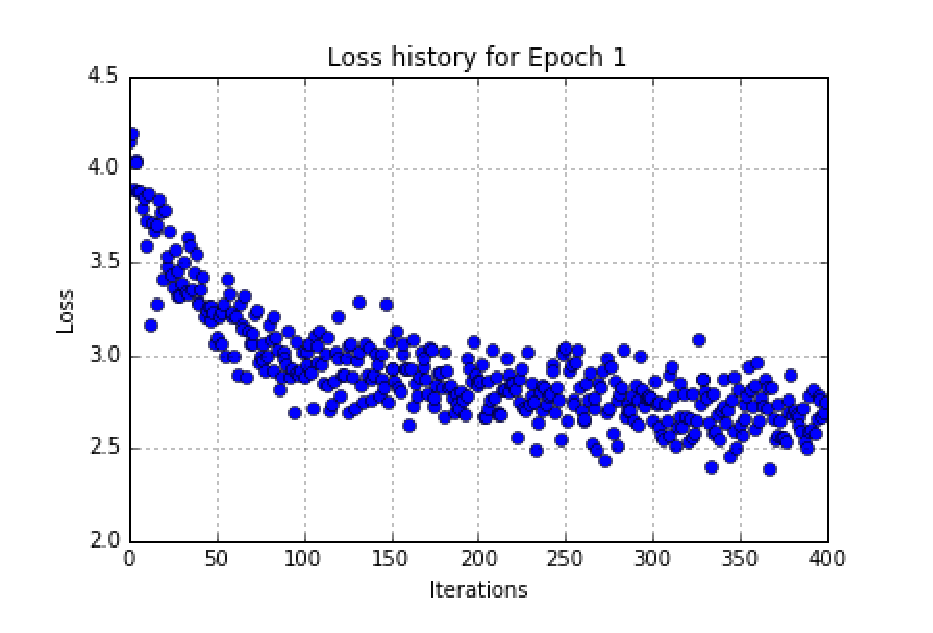
\epsfig{file=Figs4Paper/_final/convnet_losshist_epoch1.eps, height=1.5in, width=2.5in}
  \caption{Reduction in loss over several mini-batches in the first epoch of the convolutional network}
  \label{fig:lossepoch1}
\end{figure}

Figure~\ref{fig:lossepoch1} shows the reduction in the loss over multiple iterations in the first epoch. We see the loss reduces very sharply in the beginning, and then flattens out gradually.  

\begin{figure}[h!]
\centering
  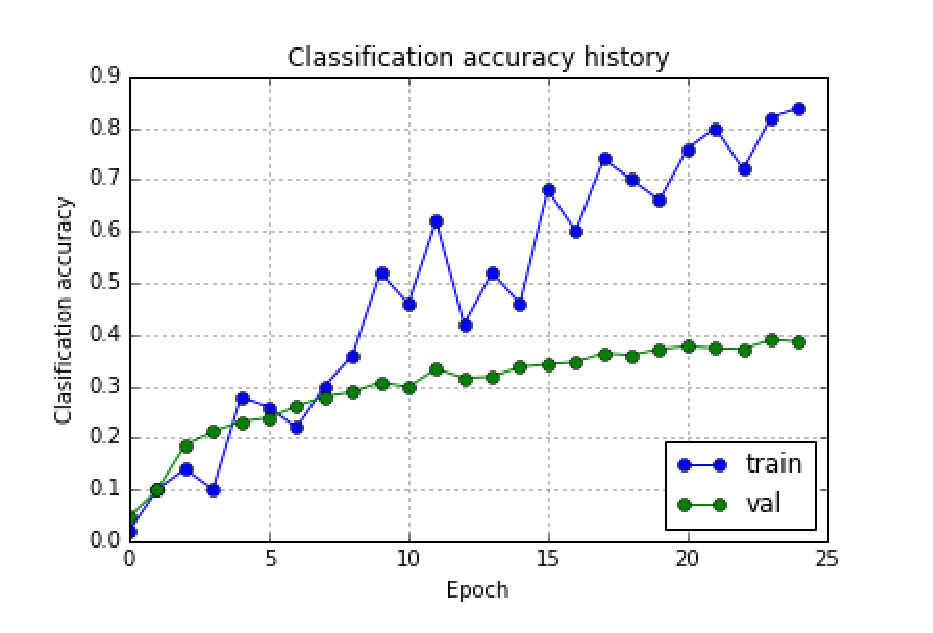
\epsfig{file=Figs4Paper/_final/convnet_classificationaccuracy.eps, height=1.5in, width=2.5in}
  \caption{Classification accuracy history of the convolutional network over 25 epochs}
  \label{fig:convnetclassificationaccuracy}
\end{figure}

Figure~\ref{fig:convnetclassificationaccuracy} shows the classification loss history for the training and validation sets over 25 epochs of the conv net.

\subsection{Transfer Learning}
\label{subsec:transferlearning}

\begin{figure}[h!]
\centering
  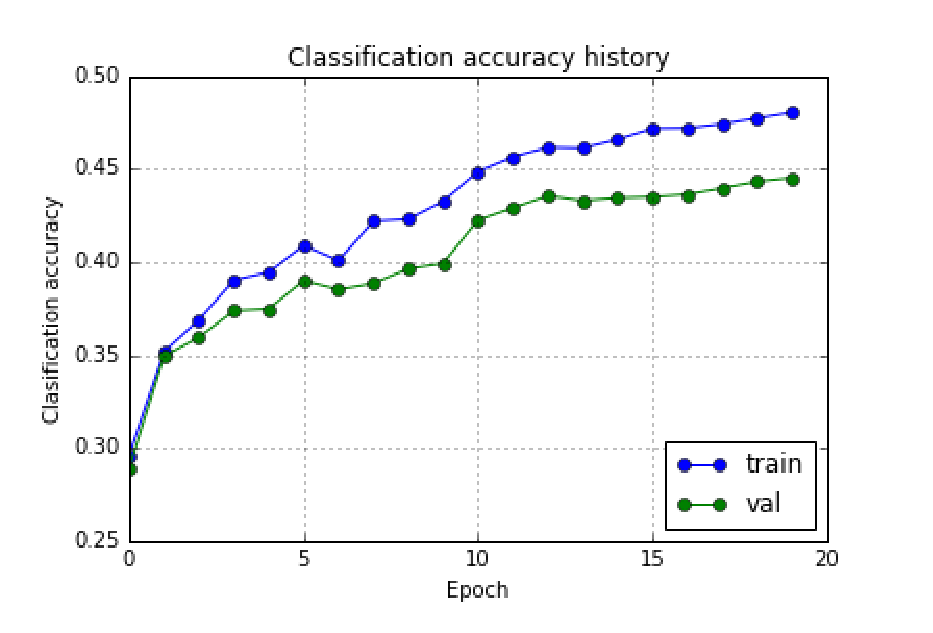
\epsfig{file=Figs4Paper/_final/transferlearning.eps, height=1.5in, width=2.5in}
  \caption{Classification accuracy history after fine-tuning a VGG model}
  \label{fig:transferlearning}
\end{figure}

To improve the accuracy of our model further, we did a set of experiments around transfer learning. Interestingly this gave us the best results on our dataset.  Some salient observations from this approach are as follows:

\begin{itemize}[noitemsep]
\item We are using the VGG-16~\cite{simonyan2014very} model pretrained on ImageNet
\item We remove the last fully connected layer (fc8) and replace it with our own, with output size 20
\item We first train the last layer for 10 epochs. This allows us to get meaningful weights for the fc8 layer first.  Subsequently, we train the entire model on our dataset for 10 more epochs.
\end{itemize}

For this approach, we referenced the TensorFlow finetune sample on GitHubGist~\cite{finetunegithubgist}. Following the example in the gist, we did similar pre-processing on our dataset to make it work for the VGG-16 model. The pre-processing steps are listed below:

\begin{itemize}[noitemsep]
\item Resize the image so its smaller side is 256 pixels long. Recall that our existing dataset has dimensions (32, 32, 3).
\item Take a random 224x224 crop of the scaled image (for the train, validation and test sets)
\item Horizontally flip the image with probability 1/2 (for the train set only)
\item Substract the per color mean VGG\_MEAN [123.68, 116.78, 103.94) (for the train, validation and test sets)
\end{itemize}


Figure~\ref{fig:transferlearning} shows the classification loss history for the training and validation sets over all the 20 epochs. Table~\ref{table:accuracyresults} shows a summary of results across different modeling approaches.





\section{Conclusion}
\label{sec:conclusion}

In this paper we propose ECNet, a hierarchical model for machine comprehension, with focus on early attention and local convolution. The goal is to use attention early in the modeling stack, and to capture local interactions using convolution layers. On the SQuAD 2.0 dataset, ECNet outperforms the BiDAF \cite{seo2016bidirectional} model proposed recently in literature.  Ablation analyses demonstrate the effect of both the novelties proposed in the model. Future work involves extending ECNet to incorporate pre-trained contextual embeddings (PCE) in the embedding layer. 



%------------------------------------------------------------------------
{\small
\bibliographystyle{ieee}
\bibliography{egbib}
}

\end{document}
